\documentclass[a4paper]{article}

%image insertion
\usepackage{graphicx} %image settings
\DeclareGraphicsExtensions{.pdf,.png,.jpg}

%math
\usepackage{amsmath} %math
%\usepackage{cmbright} %math font

%font
\usepackage{kotex}
\usepackage{fontspec}
\ifx가가
\setmainhangulfont[Ligatures=TeX,
BoldFont={KoPubBatang Medium}]{KoPubBatang Light}
\setsanshangulfont[Ligatures=TeX,
BoldFont={KoPubDotum Medium}]{KoPubDotum Light}
\setmainhanjafont[Ligatures=TeX,
BoldFont={KoPubBatang Medium}]{KoPubBatang Light}
\setsanshanjafont[Ligatures=TeX,
BoldFont={KoPubDotum Medium}]{KoPubDotum Light}
\xetexkofontregime[puncts=prevfont, colons=prevfont, cjksymbols=hangul]{latin}
\fi

%줄간격
\usepackage{setspace}
\usepackage{indentfirst}
\setstretch{1.4}
\everydisplay{\setstretch{1.2}}

%subfigure
\usepackage{subfigure}

\pagestyle{plain}
\title{물리 실험보고서 2}
\author{이한빈, 의예과 2016-XXXXX}

\begin{document}


\numberwithin{equation}{section}
\maketitle

\section{Introduction}


	축전기는 전하를 저장하는 장치로 전압이 가해졌을 때 전압에 비례하는 양의 전하를 축적한다.
		\begin{equation} \label{eq:qcv}
			Q=CV
		\end{equation}
	(\ref{eq:qcv})에 쓰인 비례상수 C는 축전기의 기하학적 모양에 의존한다. 본 실험에 쓰여진 평행판 축전기의 경우 극판의 면적이 $A$, 극판의 간격이 $d$일 때 다음으로 주어진다.
		\begin{equation} \label{eq:ppl}
			C=\epsilon_{0} \frac{A}{d} \quad (단, \: \epsilon_{0}는 \: 진공에서의 \: 유전상수)
		\end{equation}



	위치의 미소 변화 $d\vec{r}$에 대해 위치에너지의 변화가 없을 경우($dU=0$) 위의 식으로부터 $\vec{E}\bot{}d\vec{r}$임을 알 수 있다. 따라서 각 점에서의 전기장을 연결한 전기장선과 퍼텐셜이 같은 점을 이은 등전위선은 수직하게 교차한다.

		\begin{figure}[htbp]
			\begin{center}
			    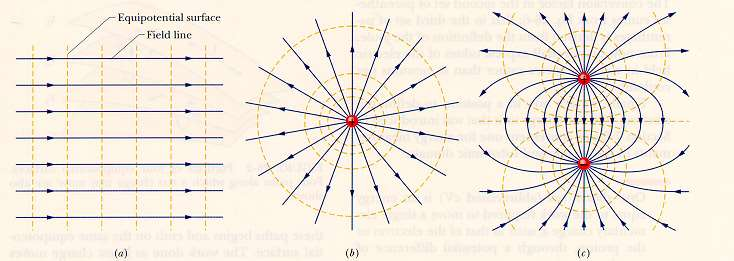
\includegraphics[width=\textwidth]{img/electircfield.png}
    			\caption{수직하게 교차하는 등전위선과 전기장선} \label{fig:ex1}
			\end{center}
		\end{figure}

	자유전자가 풍부한 도체에서는 전기장에서 평형을 이뤘을 때 모든 전하가 표면에 위치하고 내부 전기장은 0이 된다. 따라서 도체 주변의 전기력선은 도체 표면에 수직하게 들어간다.
\newpage

		\begin{figure}[htbp]
			\begin{center}
    			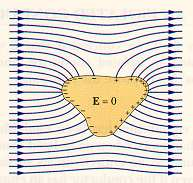
\includegraphics[width=0.5\textwidth]{img/dochae.png}
    			\caption{금속표면과 수직한 전기장선} \label{fig:ex2}
			\end{center}
		\end{figure}

	본 실험에서는 $+$와 $-$극에 사이의 전위를 측정하여 등전위선의 존재를 확인하고 전극의 모양에 따라 등전위선의 모양이 어떻게 달라지는 지 알아봤다.

\section{Method}
	\subsection{점전극}
		준비물: 컴퓨터, 점 모양 나사전극, 전위발생판   

		전위발생판 전압은 최소, 프로그램의 전위간격은 $0.3V$으로 맞춘 후 프로그램 화면을 보면서 전극과 전극 사이의 모든 등전위선을 그린다. 전압을 중간, 최대로 맞춘 후 이 과정을 반복한다. 

	\subsection{막대전극}
		준미물: 컴퓨터, 막대 모양 나사전극, 전위발생판

		전위 발생판 전압은 최대, 프로그램의 전위간격은 $0.5V$으로 맞춘 후 프로그램 화면을 보면서 전그과 전극 사이의 모든 등전위선을 그린다.

\newpage

\section{Result}
	\subsection{점전극}

		\begin{figure}[h]
				\centering
					\subfigure[Minimum Voltage]{
					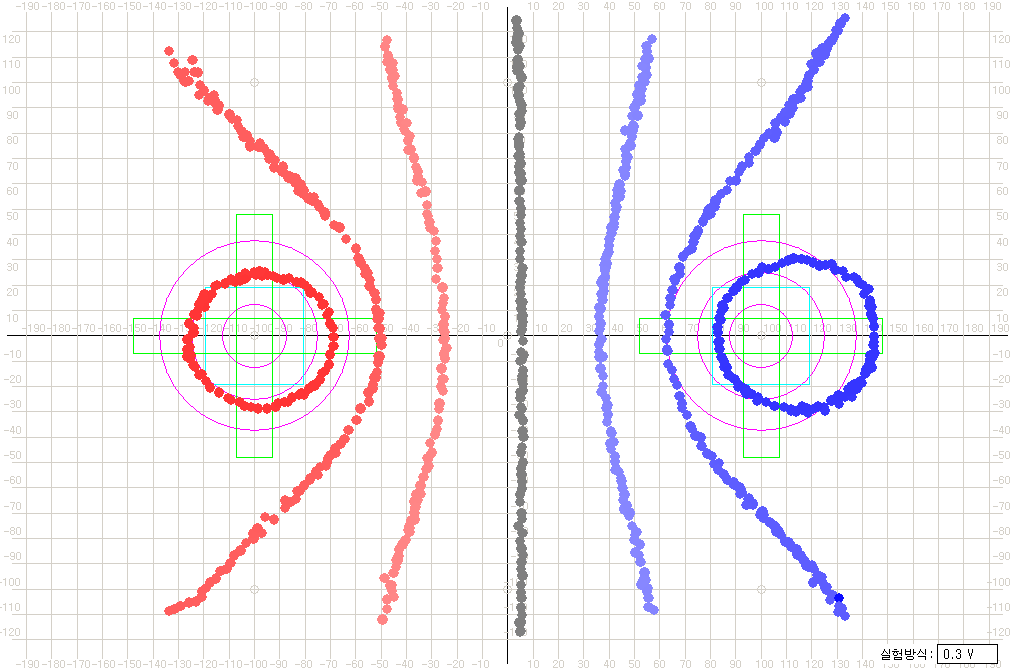
\includegraphics[width=0.4\textwidth]{img/electircfield0.png}
					\label{fig:subfig1}
					}
				\quad
					\subfigure[Midium Voltage]{
					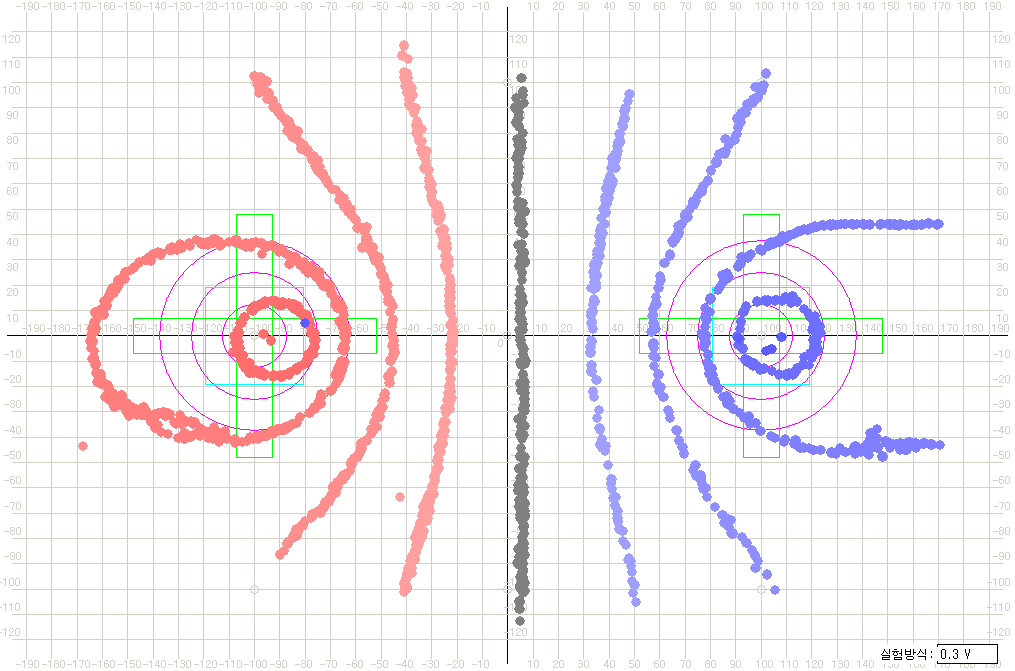
\includegraphics[width=0.4\textwidth]{img/electircfield1.png}
					\label{fig:subfig2}
					}
				\\
					\subfigure[Maximum Voltage]{
					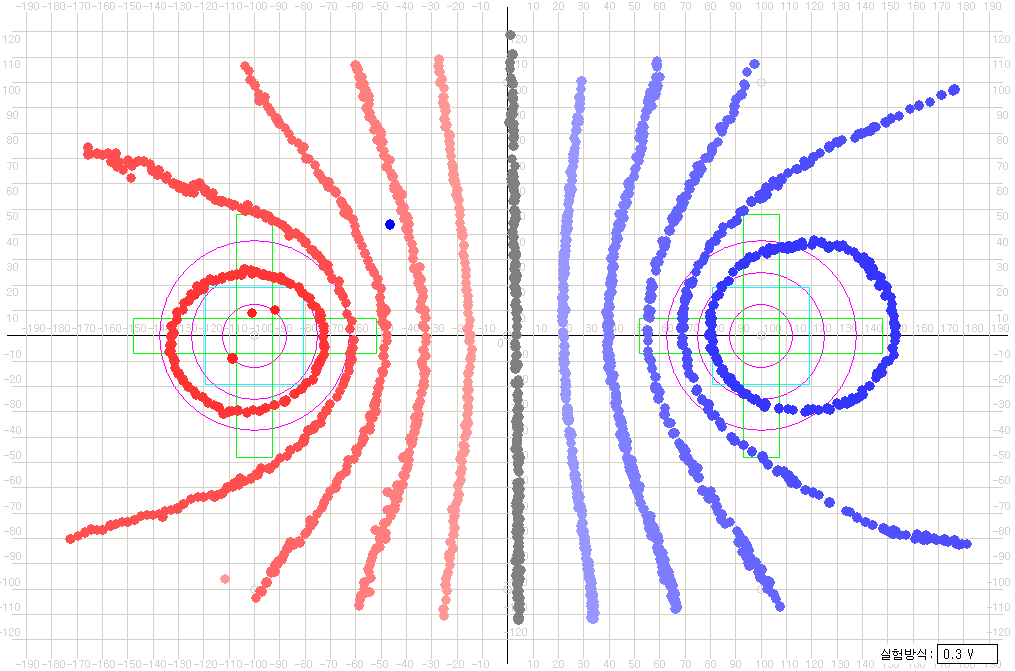
\includegraphics[width=0.4\textwidth]{img/electircfield2.png}
					\label{fig:subfig3}
					}
			\caption{Three experiments with point electrode with different voltages}
		\end{figure}	

		전압이 높아짐에 따라 등전위선의 간격이 촘촘해지는 것을 관찰할 수 있다. 전극 중간에는 등전위선이 쌍곡선 형태를 띠고 전극 가까이에서는 타원 형태를 띤다.  

	\subsection{막대전극}

		\begin{figure}[h]
			\begin{center}
				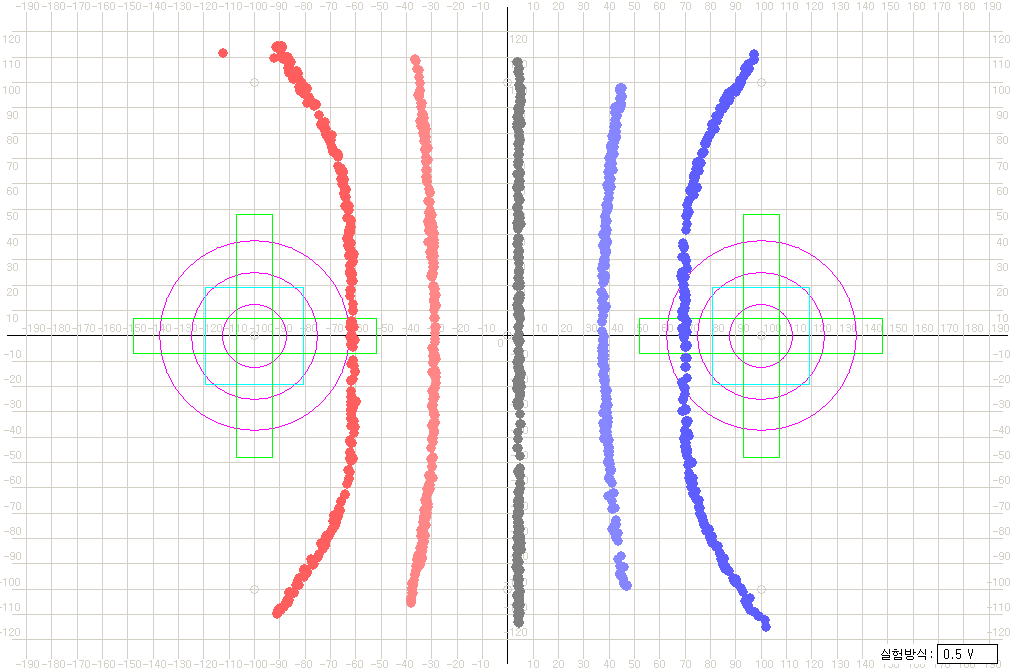
\includegraphics[width=0.4\textwidth]{img/electircfield-3.png}
				\caption{Experiment with rod electorde} \label{fig:fig4}
			\end{center}
		\end{figure}

		전극 사이에서 등전위선이 평행함을 할 수 있다. 전극 밖으로 벗어나면 전극을 둘러싸는 형태로 등전위선이 휘어짐을 관찰할 수 있다.
\newpage

\section{Conclusion}
	
	첫 번째 실험의 두 결과를 비교하면 입력 전압을 높였을 때 등전위선의 간격이 좁아짐을 관찰할 수 있었다. 거리는 유지되지만 두 극사이의 전위차가 커짐에 따라 전위차를 일정하게 설정해놓은 등전위선의 밀도가 증가하는 것이다. 이는 등전위선의 밀도가 클수록 전기장이 강하다는 사실과 부합한다.

	첫 번째 실험에서 두 극의 중간 근처에서는 등전위선의 모양이 쌍곡선 형태로 나타났다. 이는 두 극 중간 근처에서 등전위선의 간격이 일정하게 나타났다는 점과 등전위선 및 쌍곡선의 정의로부터 알아낼 수 있다. 등전위선의 간격이 일정하다는 것은 등전위선위의 점에서 각 극까지의 거리와 전위가 선형적인 관계를 가진다는 것이다. 이 때, 쌍곡선은 두 지점에서의 거리 차가 일정한 점들의 집합이라는 사실로부터 등전위선은 두 극에서 전위 차가 일정한 점들의 집합이라는 것을 알 수 있다.

	극에 가까워질수록 등전위선의 형태가 쌍곡선과 멀어진다. 이는 등전위선의 간격이 급격하게 좁아지는 것으로부터 알 수 있다. 등전위선의 간격이 일정하게 유지되지 않고 전위와 극사이의 선형적인 관계가 없어짐에 따라서 첫 번재 문단에서 얘기한 규칙이 깨지기 때문이다. 더불어 극 근처에서는 한 쪽 극의 영향이 지배적이나 반대쪽 극의 영향 떄문에 비대칭적인 원형을 띄게 된다.

	두 번째 실험에서 등전위선은 양 극판 사이에서는 극판과 평행하고 극판 밖에서는 극판을 둘러싸는 형태를 띄었다. 이는 극판을의 형태를 따라서 등전위면이 형성된다는 것이므로 극판의 성분인 금속의 표면이 전기장 속에서 등전위면을 형성한다는 사실과 일치한다.

	마지막으로 각각의 실험에서 동전을 전기장 속에 놓고 주변에서 등전위선의 형태를 측정하고자 했으나 동전이 고정이 되지 않아서 정확한 측정을 하지 못했다. 또, 장치의 입력을 최대, 등전위선 간격을 최소로 설정했음에도 등전위선의 형태변화를 얻을 수 없었다. 이를 개선하기 위해서는 더 높은 출력을 가진 장치가 필요할 것으로 생각된다. 

\section{Reference}

\end{document} 

%실험에서 개선할 점 등 피피티에서 봤던 거 모두 적어서 처리합시다.
